\chapter{Méthode CDLOD}
  \label{chap:cdlod}

  La méthode \emph{CDLOD}, pour "Continuous Distance-Dependent Level of Detail for Rendering Heightmaps" (Niveau de détail continu dépendant de la distance pour le rendue de carte de hauteur") par Filip Strugar~\cite{CDLOD}, 
  est un algorithme qui comme son nom l'indique, se base sur la distance entre la caméra et le terrain pour l'affichage du niveau de détail 
  (\textit{LOD}) basé sur une carte de hauteur (\emph{heightmap}).

  De nombreux algorithme se servent de niveaux de détail pour générer leurs terrains. Mais, un de leurs problèmes majeurs est la gestion de la séparation entre deux niveaux de détail voisins.
  
 \begin{wrapfigure}[18]{r}{6cm}
 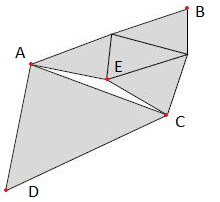
\includegraphics[width=6cm]{img/cracks.png}
   \caption[Discontinuité]{Discontinuité\protect\footnotemark}
   \label{fig:cracks}
 \end{wrapfigure}
 \footnotetext{Extrait de \url{https://people.eecs.berkeley.edu/~sequin/CS284/LECT09/L13.html}, dernier accès Mars 2018}
 
 \vspace{0.1cm}
 En effet la différence d'élévation entre chaque divisions peuvent provoquer une discontinuité dont résulte un trou. Sur la figure\ref{fig:cracks}, en se plaçant par exemple, dans le contexte d'une sphère lisse,lorsque le niveaux de détails formé par le triangle ABC se divise en 4,pour améliorer le niveau de détails de ce dernier.Le point E, formé par le changement de niveau de détail, va venir se placer à la hauteur qui lui correspond (ici en s'élevant).Un nouveau triangle se crée alors entre les sommets communs des 2 niveaux de détails voisins et le nouveau points ajuster à sa hauteur(Ici AEC).Comme ce triangle n'est pas le résultat d'une séparation/divisions d'un autre triangle, il ne possède pas de texture et crée ainsi un trou.\\
 
 
 La méthode utilisée en général pour palier à cette discontinuité est de rajouter des connexions entre les niveaux affectés. 
 Cette solution a de nombreux inconvénients, en rajoutant des connexions de cette manière, lors du rendu et, lors du parcours du terrain, ces connexions vont alors apparaître brusquement perturbant ainsi la continuité. À cela viennent s'ajouter la possibilité d'avoir des connexions multiple superposées et un coût supplémentai te en terme de calcul, mémoire et vitesse de rendu.
 
 L'algorithme CDLOD va notamment se différencier ici des autres algorithmes par ses "transitions fluides" entre les niveaux de détails par une méthode dite de "\textit{morphing}" dont nous reparlerons(section \ref{subsec:morphing} après avoir expliqué l'algorithme plus en détails.
 
 Pour pouvoir correctement expliqué l'algorithme il est tout d'abord nécessaire d'introduire les notions de  \textit{heightmap} ainsi que de \textit{quadtree} qui sont des éléments clef de l'algorithme.
 
  \section{Heightmap}
  \label{sec:heightmap}
  
  Une Heightmap pour "Carte de hauteur" est une image permettant dans le cadre de rendue de terrain, de représenter le relief à l'aide de la nuance de gris. On peut ainsi interpréter la nuance comme une hauteur par rapport à la surface. Le noir (une nuance nulle) représente la hauteur minimum et le blanc (une nuance maximal) représente la hauteur maximum. Des algorithmes permettent d'obtenir une carte de hauteur ressemblant à des terrains naturels. Comme par exemple, l'algorithme de bruit de perlin~\cite{Perlin}, bruit de simplex , déplacement du point médian...
  
  
  
  \section{Quadtree}
  \label{sec:quadtree}
  
\begin{wrapfigure}[12]{r}{6cm}
 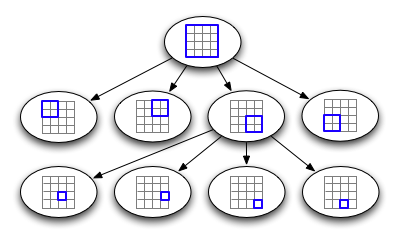
\includegraphics[width=6cm]{img/quadtree-arbre.png}
   \caption[Quadtree]{Quadtree\protect\footnotemark}
   \label{fig:quadtree-arbre}
 \end{wrapfigure}
 \footnotetext{Extrait de \url{http://codeforces.com/blog/entry/57498}, dernier accès Mars 2018}
  
 Un \emph{quadtree} est une structure de données s'apparentant à un arbre ou chaque n\oe{}ud de l'arbre possède quatre fils. Utiliser un \emph{quadtree} est un bon moyen de diviser un terrain 2D en plusieurs région (représenter ici par la figure \ref{fig:quadtree-arbre}. Le terrain d'origine peux ainsi être diviser en quatre plus petites régions égales, puis chaque régions obtenues en quatre sous-régions, et ainsi de suite, avec chaque n\oe{}ud comprenant des données correspondant à une sous-région. Pour à terme obtenir la région initial divisé en $4^n$ plus petite région de même taille avec n la hauteur de l'arbre.

  
\vspace{1.5cm}

\section{Continuous Distant-Dependent LOD ****}


  La méthode \textit{CDLOD}, est basé sur la méthode \textit{CLOD} "Chuncked LOD" développé par Thatcher Ulrich~\cite{CLOD} (dont nous proposont un résumé en annexe \ref{sec:chunked-lod}).
  

  Cette méthode organise une \emph{heightmap} dans un \emph{quadtree}, qui est utilisé pour sélectionner les niveaux de détails nécessaire au rendu. Lors de l'exécution le \emph{quadtree} est généré et composé des niveaux de détails, les \emph{LOD} nécessaire sont calculés et ainsi utilisés depuis le \emph{quadtree}. L'algorithme va assuré que le nombre de triangles affiché à l'écran soient constant, quelle que soit la distance entre la caméra et le terrain.
  
 \subsection{Sélection des n\oe{}uds dans le Quadtree ****}
 
    Pour pouvoir assurer que le nombre de triangles affichés à l'écran reste constant, il est nécessaire d'effectuer la sélection dans le \emph{quadtree} à chaque fois que la caméra bouge.\\
    \vspace{0.5cm}
    \begin{wrapfigure}[17]{r}{6cm}
 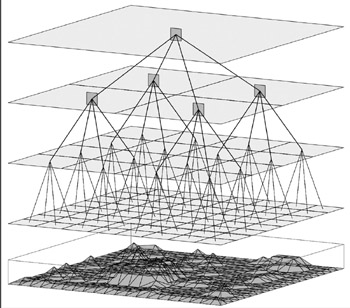
\includegraphics[width=6cm]{img/quadtree.png}
   \caption[Quadtree]{Quadtree\protect\footnotemark}
   \label{fig:quadtree-selection}
 \end{wrapfigure}
 \footnotetext{Extrait de \url{https://flylib.com/books/en/2.124.1.130/1/}, dernier accès Mars 2018}
    Le rendu du terrain est alors effectué en fonction de la distance entre le terrain et la caméra. Pour affiché un n\oe{}ud, le \emph{quadtree} est parcouru depuis la racine avec une tolérance maximum prédéfinie, permettant de savoir si le n\oe{}ud doit être affiché. Si le n\oe{}ud parcouru est suffisamment proche de la caméra il est affiché, et on vérifie si la tolérance maximum permet l'affichage de ses fils, et ainsi de suite. Les zones proches auront un niveau de détails élevé, alors que les zones plus lointaines seront moins détaillées. Le niveau de détails correspond alors à la profondeur dans le \emph{quadtree}, comme on peut l'observer sur la figure \ref{fig:quadtree-selection}

\vspace{0.5cm}

\subsection{Transitions de LOD ****}
    l'algorithme de CDLOD garde en continue un niveau de détail en utilisant sans arrêt des transitions. Contrairement à la méthode Chuncked-LOD de Ulrich.T~\cite{CLOD} , Strugar.F dans sa méthode~\cite{CDLOD}, n'utilise pas de "rideau" pour combler le vide provoqué par la différence de niveau de détail, mais s'assure que le maillage du niveau supérieur soit complètement transformé en maillage de niveau inférieur avant que la changement ne se produise. Cela signifie qu'il n'y aura aucune apparition brusque ni de discontinuité.
    
\begin{figure}[!ht]
    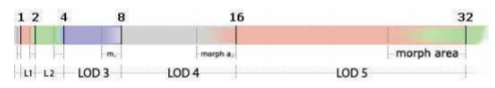
\includegraphics[width=12cm]{img/morph-area.png}
    \caption[morph-area]{Zone de transition \protect\footnotemark}
    \label{fig:morph-area}
\end{figure}
    \footnotetext{Extrait de \url{http://www.vertexasylum.com/downloads/cdlod/cdlod_latest.pdf}, dernier accès Mars 2018}
    
    La zone de transition couvre environ 15 à 30\% de chaque LOD.\\
    
    La figure \ref{fig:morph-area} montre les différents niveaux de transitions du système de morphing,
    le niveau L1 étant le niveau le plus proche de la caméra et donc le niveau avec le plus de détail.
    On peut voir que les différents niveaux de transition ne sont pas linéaire en fonction de la distance,
    les détails de la fonction de transition seront expliqué plus bas dans la partie implémentation.
    
\subsection{Morphing ****}
\label{subsec:morphing}

  L'opération de "morphing" est fait dans le vertex shader et chaque n\oe{}ud peut être transformé pour correspondre à un n\oe{}ud, soit un niveau plus élevé ou un niveau inférieur dans la quadtree. La morph est réalisée de telle manière que chaque bloc de 8 triangles sont  facilement transformé en un bloc correspondant de 2 triangles. Ce morphing se traduira par des transitions en douceur sans discontinuité.
  Lors du rapprochement(ou éloignement) de la caméra les sommets sont déplacé verticalement pour correspondre au niveau souhaité (représentation à la figure \ref{fig:morph-transition}).
\begin{figure}[!ht]
    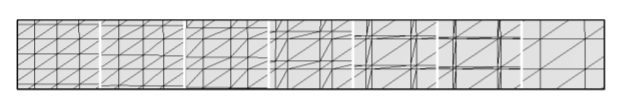
\includegraphics[width=12cm]{img/morph-transition.png}
    \caption[morph-transition]{Représentation des transitions \protect\footnotemark}
    \label{fig:morph-transition}
    \end{figure}
    \footnotetext{Extrait de \url{http://www.vertexasylum.com/downloads/cdlod/cdlod_latest.pdf}, dernier accès Mars 2018}


\subsection{Basic et Streaming Version}

    Il existe deux façons de stocker le Quadtree qui d'une version à l'autre réduit considérablement la mémoire utilisé. En effet la version BasicCDLOD assez simple à mettre en oeuvre étend et stock entièrement tout les LOD, et, va venir parcourir la structure de donnée afin de sélectionné les niveaux nécessaire.
   
    Une autre version proposé, plus complexe à mettre en oeuvre mais qui économise grandement la mémoire, est la méthode StreamingCDLOD où seuls les parties nécessaires à la vue actuelle sont conservés. Les n\oe{}uds sont ensuite permutées si nécessaire. Par conséquent, les n\oe{}uds qui n'ont pas été utilisé pendant un certain temps peuvent être libérés.